\documentclass[aspectratio=43]{beamer}
\usepackage[latin1]{inputenc}
\usepackage{amsmath}
\usepackage{amsfonts}
\usepackage{amssymb}
\usepackage{makeidx}
\usepackage{graphicx}
\usepackage{array}

% Customization
\mode<presentation>{
%	\usetheme{CambridgeUS}
%	\usecolortheme{dolphin}
	\setbeamertemplate{navigation symbols}{}
	%     \usetheme{Frankfurt}
	%     \usetheme{Madrid}
	%     \usetheme{Warsav}
}
\setbeamertemplate{footline}[frame number]

%TikZ diagrams
\usepackage{tikz}
\usetikzlibrary{patterns}
\usetikzlibrary{arrows,shapes}
\usetikzlibrary{shapes.multipart}
\usetikzlibrary{trees}
\usetikzlibrary{shapes.geometric}
\usetikzlibrary{matrix,arrows}
\usetikzlibrary{positioning}
\usetikzlibrary{calc,through}
\usetikzlibrary{decorations.pathreplacing}
\usepackage{pgffor}

% Define colors
\definecolor{darkgreen}{rgb}{0.0, 0.5, 0.13}
\definecolor{darkblue}{rgb}{0.0, 0.0, 0.55}
\definecolor{darkred}{rgb}{0.55, 0.0, 0.0}

% For using TikZ
\usetikzlibrary{decorations.pathmorphing}
\usetikzlibrary{decorations.markings}
\tikzset{
	vector/.style={decorate, decoration={snake,amplitude=3pt}, draw},
	gluon/.style={decorate, decoration={coil,amplitude=2.5pt},draw},
	provector/.style={decorate, decoration={snake,amplitude=2.5pt}, draw},
	antivector/.style={decorate, decoration={snake,amplitude=-2.5pt}, draw},
	fermion/.style={draw=black, postaction={decorate},
		decoration={markings,mark=at position .55 with {\arrow[draw=black,thick]{>}}}},
	fermionbar/.style={draw=black, postaction={decorate},
		decoration={markings,mark=at position .55 with {\arrow[draw=black,thick]{<}}}},
	fermionnoarrow/.style={draw=black},
	gluon/.style={decorate, draw=black,
		decoration={coil,amplitude=2.5pt, segment length=3pt}},
	gluon2/.style={decorate, draw=black,
		decoration={coil,amplitude=1.75pt, segment length=2.75pt}},
	scalar/.style={dashed,draw=black, postaction={decorate},
		decoration={markings,mark=at position .55 with {\arrow[draw=black]{>}}}},
	scalarbar/.style={dashed,draw=black, postaction={decorate},
		decoration={markings,mark=at position .55 with {\arrow[draw=black]{<}}}},
	scalarnoarrow/.style={dashed,draw=black},
	electron/.style={draw=black, postaction={decorate},
		decoration={markings,mark=at position .55 with {\arrow[draw=black]{>}}}},
	bigvector/.style={decorate, decoration={snake,amplitude=4pt}, draw},
}

% Blocks
\tikzstyle{block} = [draw, rectangle, minimum height = 3em, rounded corners, minimum width = 4em]
\tikzstyle{block2} = [draw, rectangle, minimum height = 3em, rounded corners, minimum width = 7em]
\tikzstyle{circle} = [draw, circle, radius = 1.5]
\tikzstyle{arrow} = [thick,->]
%************************************************************************************************************

% Title and author
\title{A new generation of PDFs with deep learning models}
\author{\textbf {Jesus Urtasun Elizari}}
\institute{\textbf {University of Milan}}
\date{Cambridge, 26 july 2012}

\begin{document}

% 1. Front slide
\begin{frame}

	\center{\color{blue}A new generation of PDFs with deep learning models}
	\center{\color{blue}Operator implementation in TensorFlow}

	\center{Jesus Urtasun Elizari, University of Milan}
	\center{Cambridge, June 2019}

	\begin{figure}
		\minipage{1\textwidth}
		\includegraphics[width = 2.5 cm]{n3pdf.png}
		\hfill
		\includegraphics[width = 2.5 cm]{unimi.png}
		\hfill
		\includegraphics[width = 2.5 cm]{erc.png}
		\endminipage
	\end{figure}

\end{frame}

% Introduction
\begin{frame}

	\frametitle{Outline}
	
	\begin{enumerate}
		\item Introduction. General structure of a process.
		\item Structure of {\color{violet}n3fit}. Motivation for operator implementation.
		\item Operator implementation in TensorFlow.
		\item Results $\&$ Conclusions.
	\end{enumerate}
	
\end{frame}

% Deep Inelastic Scattering
\begin{frame}

	\frametitle{General structure of a process}
	\framesubtitle{Deep Inelastic Scattering}

	\begin{figure}
		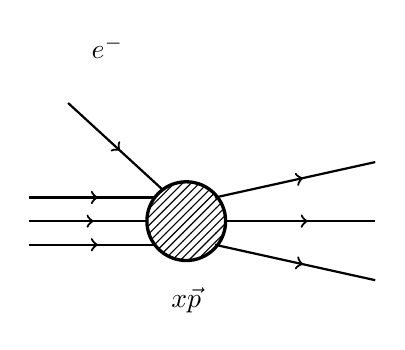
\begin{tikzpicture}
			% Incoming fermions
			\draw [thick, fermion] (-3.5, -0.5)--(-2.3, -1.6);
			\draw [thick, fermion] (-4, -1.7)--(-2.4, -1.7);
			\draw [thick, fermion] (-4, -2)--(-2.5, -2);
			\draw [thick, fermion] (-4, -2.3)--(-2.4, -2.3);
			\draw [thick, very thick, pattern = north east lines] (-2, -2) circle [radius = 0.5];
			\node at (-2.0, -3.0) {$x\vec{p}$};
			% Outcoming fermions
			\draw [thick, fermion] (-1.635, -1.7)--(0.4, -1.25);
			\draw [thick, fermion] (-1.5, -2)--(0.4, -2);
			\draw [thick, fermion] (-1.635, -2.3)--(0.4, -2.75);
			% Labels
			\node at (-3, 0.2) {$e^{-}$};
			% Braces
			
			
		\end{tikzpicture}
	\end{figure}

	Convolute the partonic $\hat{\sigma}_{i j}$ with the PDF $\longrightarrow$ Observable $\sigma$.
	\begin{equation}
		\sigma^{DIS} = \int_{0}^{\infty} dx \; f_{\alpha}(x) \ast \hat{\sigma}_{i j}(\mu_{F}, \mu_{R}(\alpha_{s})) \; .
	\end{equation}
	In our language $\longrightarrow$ vector of observables from a grid of $x_{i}$:
	\begin{equation}
		y_{N}^{DIS} = \sum_{i, \alpha} f_{\alpha}(x_{i}) FK_{N i \alpha} \; .
	\end{equation}
	
\end{frame}

% 5. Drell-Yan
\begin{frame}

	\frametitle{General structure of a process}
	\framesubtitle{Hadronic (Example: Drell-Yan)}
	
	\begin{figure}
		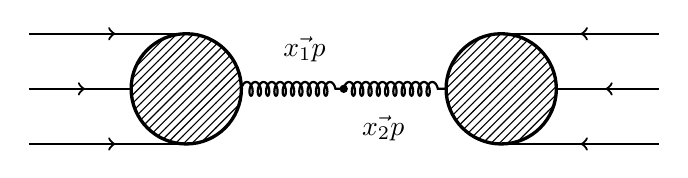
\begin{tikzpicture}
			% Incoming first proton 
			\draw [thick, fermion] (-4, 0.7)--(-2, 0.7);
			\draw [thick, fermion] (-4, 0)--(-2.7, 0);
			\draw [thick, fermion] (-4, -0.7)--(-2, -0.7);
			\draw [thick, very thick, pattern = north east lines] (-2, 0) circle [radius = 0.7];
			% Gluons
			\draw [thick, gluon] (-1.3, 0)--(0, 0);
			\draw [thick, gluon] (0, 0)--(1.3, 0);
			\node at (-0.5, 0.5) {$\vec{x_{1}p}$};
			\node at (0.5, -0.5) {$\vec{x_{2}p}$};
			\draw [thick, very thick, fill = black, pattern = north east lines] (0, 0) circle [radius = 0.03];
			% Incoming second proton
			\draw [thick, very thick, pattern = north east lines] (2, 0) circle [radius = 0.7];
			\draw [thick, fermionbar] (2, 0.7)--(4, 0.7);
			\draw [thick, fermionbar] (2.7, 0)--(4, 0);
			\draw [thick, fermionbar] (2, -0.7)--(4, -0.7);
		\end{tikzpicture}
	\end{figure}

	Convolute the partonic $\hat{\sigma}_{i j}$ with the PDF $\longrightarrow$ Observable $\sigma$.
	\begin{equation}
		\sigma^{DY} = \int_{0}^{\infty} dx_{1} \; dx_{2} \; f_{\alpha}(x_{1}) \ast f_{\beta}(x_{2}) \ast \hat{\sigma}_{i j}(\mu_{F}, \mu_{R}(\alpha_{s})) \; .
	\end{equation}
	In our language $\longrightarrow$ vector of observables from a grid of $x_{i}$:
	\begin{equation}
		y_{N}^{DY} = \sum_{i, j, \alpha, \beta} f_{\alpha}(x_{i}) f_{\beta}(x_{j}) FK_{N i j \alpha \beta} \; .
	\end{equation}
	{\color{blue} Note: We will use DY to refer hadronic events}
\end{frame}

% General structure of the model
\begin{frame}

	\frametitle{General structure of the model}
	\framesubtitle{General structure of n3fit}

	\begin{figure}
		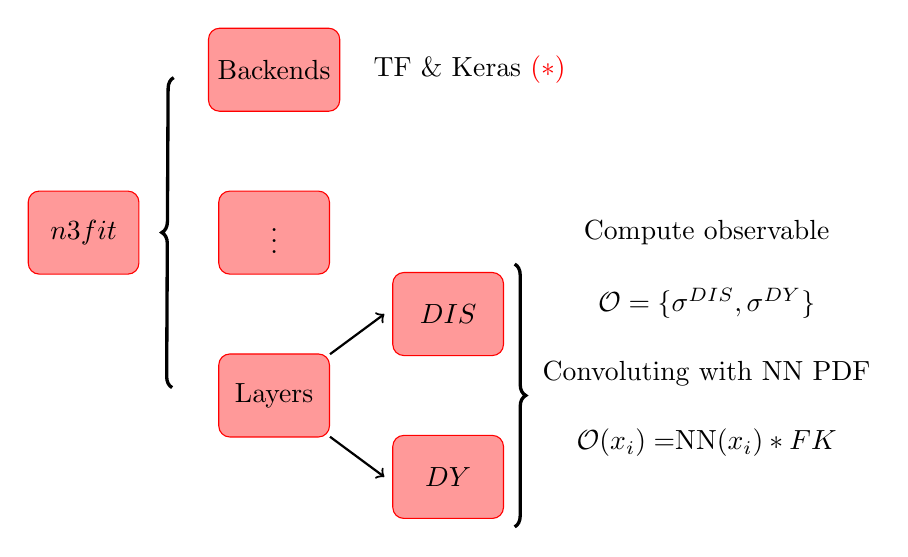
\begin{tikzpicture}
			
			%List of boxes composing n3fit
			\node[block, draw = red, fill = red!40] (n3fit) {$n3fit$};
			\node[block, draw = red, fill = red!40, right = 1.0cm of n3fit] (runcards) {\vdots};
			\node[block, draw = red, fill = red!40, above = 1.0cm of runcards] (backends) {Backends};
			\node[block, draw = red, fill = red!40, below = 1.0cm of runcards] (layers) {Layers};
			\node[right = 0.3 cm of backends] (keras) {TF $\&$ Keras {\color{red}($\ast$)}};
			\coordinate[right = 1.5 cm of layers] (rlayer);
			
			% Brace
			\coordinate[left = 0.5 cm of backends] (lbackend);
			\coordinate[left = 0.65 cm of layers] (llayer);
			\draw[decorate, decoration = {brace, amplitude = 4pt, raise = 1pt}, very thick]
			($(llayer.south west) + (0.1, 0.1)$) -- ($(lbackend.north west) + (0.1,-0.1)$);
			
			% Layers DIS and DY
			\node[block, draw = red, fill = red!40, above = 0.5 cm of rlayer] (DIS) {$DIS$};
			\node[block, draw = red, fill = red!40, below = 0.5 cm of rlayer] (DY) {$DY$};
			\coordinate[left = 0.1 cm of DIS] (lDIS);
			\coordinate[left = 0.1 cm of DY] (lDY);
			
			% Connect all nodes defined above
			\draw[arrow] (layers) -- (lDIS);
			\draw[arrow] (layers) -- (lDY);
			
			% Braces
			\draw[decorate, decoration = {brace, amplitude = 4pt, raise = 1pt}, very thick]
			($(DIS.north east) + (0.1, 0.1)$) -- ($(DY.south east) + (0.1,-0.1)$);
			
			% Implement in n3fit
			\node[right = 3.1 cm of runcards] (obs) {Compute observable};
			\node[below = 0.3 cm of obs] (obs2) {$\mathcal{O} = \{ \sigma^{DIS}, \sigma^{DY} \}$};
			\node[below = 0.3 cm of obs2] (obs3) {Convoluting with NN PDF};
			\node[below = 0.3 cm of obs3] (obs4) {$\mathcal{O}(x_{i}) = $NN$(x_{i}) \ast FK$};
		
		\end{tikzpicture}
	\end{figure}

\end{frame}

% 8. Operator implementation
\begin{frame}

	\frametitle{Operator implementation}
	\framesubtitle{i) General structure of observable layers}
	
	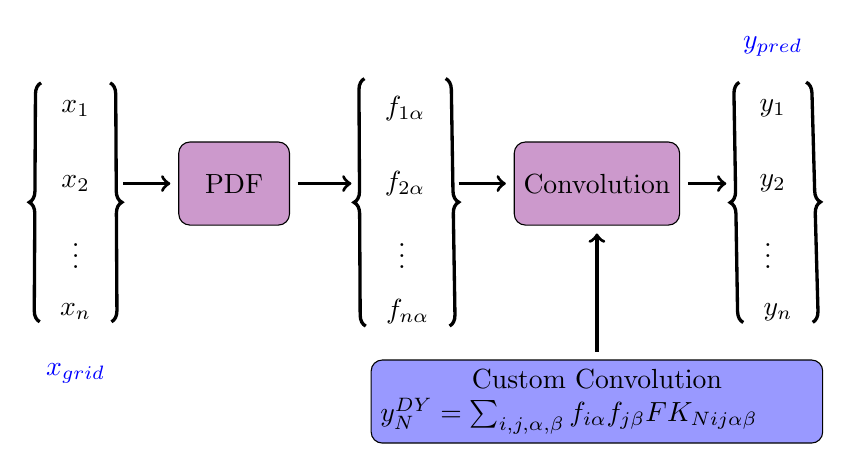
\begin{tikzpicture}
	
		% List of xs
		\node (x1) {$x_{1}$};
		\node[below = 0.5 cm of x1] (x2) {$x_{2}$};
		\node[below = 0.2 cm of x2] (xd) {\vdots};
		\node[below = 0.2 cm of xd] (xn) {$x_{n}$};
		\node[below = 0.3 cm of xn] (xgrid) {\color{blue}$x_{grid}$};
		\coordinate[right = 0.3 cm of x2] (rx2);
		% Braces
		\draw[decorate, decoration={brace, amplitude = 4pt, raise = 1pt}, very thick]
		($(x1.north east) + (0.1, 0.1)$) -- ($(xn.south east) + (0.1, 0.1)$);
		\draw[decorate, decoration={brace, amplitude = 4pt, raise = 1pt}, very thick]
		($(xn.south west) + (-0.1, 0.1)$) -- ($(x1.north west) + (-0.1, 0.1)$);
		
		% PDF layer
		\node[block, fill = violet!40, right = 1.0 cm of x2] (pdf) {PDF};
		\coordinate[left = 0.1 cm of pdf] (lpdf);
		\coordinate[right = 0.1 cm of pdf] (rpdf);
		
		% List of pdfs
		\node[right = 3.5 cm of x1] (f1) {$f_{1 \alpha}$};
		\node[right = 3.5 cm of x2] (f2) {$f_{2 \alpha}$};
		\node[right = 3.8 cm of xd] (fd) {\vdots};
		\node[right = 3.5 cm of xn] (fn) {$f_{n \alpha}$};
		\coordinate[left = 0.3 cm of f2] (lf2);
		\coordinate[right = 0.3 cm of f2] (rf2);
		% Braces
		\draw[decorate, decoration = {brace, amplitude = 4pt, raise = 1pt}, very thick]
		($(f1.north east) + (0.1, 0.1)$) -- ($(fn.south east) + (0.1, 0.1)$);
		\draw[decorate, decoration = {brace, amplitude = 4pt, raise = 1pt}, very thick]
		($(fn.south west) + (-0.1, 0.1)$) -- ($(f1.north west) + (-0.1, 0.1)$);
		
		% Convolution layer
		\node[block, fill = violet!40, right = 1.0 cm of f2] (conv) {Convolution};
		\coordinate[left = 0.1 cm of conv] (lconv);
		\coordinate[right = 0.1 cm of conv] (rconv);
		\coordinate[below = 0.1 cm of conv] (bconv);
		
		% Custom Convolution 
		\node[block, fill = blue!40, below = 1.7 cm of conv, text width = 5.5 cm] (myconv) {\centering Custom Convolution \\ $y_{N}^{DY} = \sum_{i, j, \alpha, \beta} f_{i \alpha} f_{j \beta} FK_{N i j \alpha \beta}$};
		\coordinate[above = 0.1 cm of myconv] (amyconv);
		
		% List of y
		\node[right = 4.0 cm of f1] (y1) {$y_{1}$};
		\node[right = 4.0 cm of f2] (y2) {$y_{2}$};
		\node[right = 4.3 cm of fd] (yd) {\vdots};
		\node[right = 4.0 cm of fn] (yn) {$y_{n}$};
		\node[above = 0.3 cm of y1] (ypred) {\color{blue}$y_{pred}$};
		\coordinate[left = 0.3 cm of y2] (ly2);
		% Braces
		\draw[decorate, decoration = {brace, amplitude = 4pt, raise = 1pt}, very thick]
		($(y1.north east) + (0.1, 0.1)$) -- ($(yn.south east) + (0.1, 0.1)$);
		\draw[decorate, decoration = {brace, amplitude = 4pt, raise = 1pt}, very thick]
		($(yn.south west) + (-0.1, 0.1)$) -- ($(y1.north west) + (-0.1, 0.1)$);
			
		% Connect all nodes defined above
		\draw[arrow, very thick] (rx2) -- (lpdf);
		\draw[arrow, very thick] (rpdf) -- (lf2);
		\draw[arrow, very thick] (rf2) -- (lconv);
		\draw[arrow, very thick] (rconv) -- (ly2);
		\draw[arrow, very thick] (amyconv) -- (bconv);
		
	\end{tikzpicture}
	
	\begin{enumerate}
		\item Build model to compute $y_{pred}$ from $x_{grid}$
		\item Compute $\chi^{2}$ loss by comparing with data $\chi^{2} = \sum_{i = 1}^{N} y_{i}^{pred} - y_{i}^{data}$
		\item Compute gradient $\nabla \chi^{2}$ and update values of PDF $\longrightarrow$ {\color{violet} Fit}
	\end{enumerate}
\end{frame}
	
% 9. Gradient implementation
\begin{frame}

	\frametitle{Operator implementation}
	\framesubtitle{ii) TF computation of the gradient}

	\begin{enumerate} 
		\item Computing gradient of the $\chi^{2}$ with respect to all parameters of the network.
		\begin{equation}
			\nabla \chi^{2} \longrightarrow \frac{\partial \chi^{2}}{\partial x_{i}} \nonumber
		\end{equation}
		\item TF requires the gradient with respect to any operation in the model.
		\begin{equation}
			\frac{\partial \chi^{2}}{\partial x_{i}} =
			\frac{\partial \chi^{2}}{\partial \textbf{Op}}
			{\color{red}\frac{\partial \textbf{Op}}{\partial f_{\mu \nu}}} \ldots
			\frac{\partial f_{\mu \nu}}{\partial x_{i}}
		\end{equation}
		\item TF does not know the structure of \textbf{Op}. Compute manually the gradient $\frac{\partial \textbf{Op}}{\partial f_{\mu \nu}}$ and implement it in the TF framework.
	\end{enumerate}

\end{frame}

% Computation of the gradient
\begin{frame}
	
	\frametitle{Operator implementation}
	\framesubtitle{iii) Manual computation of the gradient}
	
	\begin{enumerate}
		\item From the expression of the output:
		\begin{equation}
			\textbf{Op} \equiv y_{N} = \sum_{i, j, \alpha, \beta} f_{\alpha}(x_{i}) f_{\beta}(x_{j}) FK_{N i j \alpha \beta} \nonumber
		\end{equation}
		\item Gradient of the output with respect ot the PDFs:
		\begin{align}
			\frac{\partial y_{N}}{\partial f_{\mu \nu}} &=
			\frac{\partial}{\partial f_{\mu \nu}} \sum_{i, j, \alpha, \beta} f_{i \alpha} f_{j \beta} FK_{N i j \alpha \beta} \nonumber \\
			&= \sum_{i, j, \alpha, \beta} (\delta_{\mu i} \delta_{\nu \alpha} f_{\beta j} + \delta_{\mu j} \delta_{\nu \beta} f_{\alpha i})
			FK_{N i j \alpha \beta} \\
			&= \sum_{j, \beta} f_{j \beta} FK_{N \mu j \nu \beta} + \sum_{i, \alpha} f_{i \alpha} FK_{N i \mu \alpha \nu} \nonumber
		\end{align}

	\end{enumerate}

\end{frame}

% Technical details
\begin{frame}

	\frametitle{Through technical details}
	\framesubtitle{i) Generating libraries}
	
	\begin{enumerate}
		\item Build {\color{blue}.cc} files computing the convolution and the gradient.
		\item Compile them to build {\color{darkgreen}.so} libraries. \\
		{\color{orange}g++ -std=c++11 -shared My$\_$Convolution$\_$.cc -o My$\_$Convolution$\_$.so $\$$TF$\_$FLAGS}
		\item load the libraries in DIS/DY layers of {\color{violet} n3fit} with {\color{orange} load$\_$op$\_$library()} function of TensorFlow.
	\end{enumerate}
	\begin{figure}
		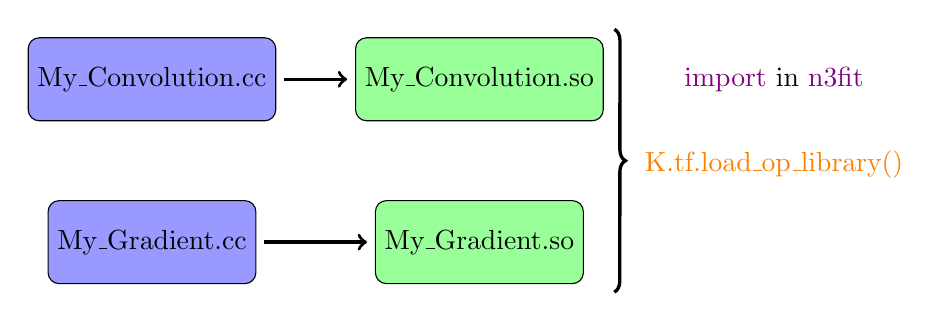
\begin{tikzpicture}
		
			% .cc files
			\node[block, fill = blue!40] (myconv) {My$\_$Convolution.cc};
			\coordinate[right = 0.1 cm of myconv] (rconv);
			\node[block, fill = blue!40, below = 1.0 cm of myconv] (mygrad) {My$\_$Gradient.cc};
			\coordinate[right = 0.1 cm of mygrad] (rgrad);
			
			% .so files
			\node[block, fill = green!40, right = 1.0 cm of myconv] (soconv) {My$\_$Convolution.so};
			\coordinate[left = 0.1 cm of soconv] (lsoconv);
			\node[block, fill = green!40, below = 1.0 cm of soconv] (sograd) {My$\_$Gradient.so};
			\coordinate[left = 0.1 cm of sograd] (lsograd);
			
			% Braces
			\draw[decorate, decoration = {brace, amplitude = 4pt, raise = 1pt}, very thick]
			($(soconv.north east) + (0.1, 0.1)$) -- ($(sograd.south east) + (0.35,-0.1)$);
			
			% Implement in n3fit
			\node[right = 0.9 cm of soconv] (import) { {\color{violet} import} in {\color{violet} n3fit} };
			\node[below = 0.5 cm of import] (importconv) { \color{orange} K.tf.load$\_$op$\_$library() };
			
			% Connect all nodes defined above
			\draw[arrow, very thick] (rconv) -- (lsoconv);
			\draw[arrow, very thick] (rgrad) -- (lsograd);
		
		\end{tikzpicture}
	\end{figure}

\end{frame}

% Technical details
\begin{frame}
	
	\frametitle{Through technical details}
	\framesubtitle{ii) Writing the convolution in c++}
	
	\begin{enumerate}
		\item Input PDF: $f_{i \alpha}$ and FK table: $FK_{N i j \alpha \beta}$
		\item Basis flavors: $basis = \{(1, 2), (3, 4), ..., (3, 1)\}$
		\begin{figure}
			\includegraphics[width = 0.75\textwidth]{myconvdy.png}
		\end{figure}
		\item Compute convolution $y_{N}^{DY} = \sum_{i, j, \alpha, \beta} f_{i \alpha} f_{j \beta} FK_{N i j c} \delta^{c}_{\alpha \beta}$
	\end{enumerate}
	\begin{figure}
		\includegraphics[width = 0.75\textwidth]{myconvdy2.png}
	\end{figure}

\end{frame}

% Technical details
\begin{frame}

	\frametitle{Through technical details}
	\framesubtitle{iii) Writing the observable layer}
	A DY class written in TF would need at least 3 operations
	\begin{enumerate}
		\item Generate luminosity tensor $\mathcal{L}_{i j \alpha \beta} = f_{i \alpha} \ast f_{j \beta}$
		\item Apply mask to eliminate the non-active flavors
		\item Perform the convolution $y_{N}^{DY} = \sum_{i, j, \alpha, \beta} \mathcal{L}_{i j \alpha \beta} FK_{N i j c} \delta^{c}_{\alpha \beta}$
	\end{enumerate}
		\begin{figure}
			\includegraphics[width = 0.7\textwidth]{dyclassold.png}
		\end{figure}
	Custom DY class just calls the {\color{blue}MyConvolutionDY.cc}
	\begin{figure}
		\includegraphics[width = 1.05\textwidth]{dyclass.png}
	\end{figure}

\end{frame}

%Results DIS ratio
\begin{frame}

	\frametitle{Results}
	\framesubtitle{Checking computation}
	
	{\Large DIS only:}
	\begin{table}
		\centering
		\begin{tabular}{c c c c}
			& TensorFlow & Custom & Ratio \\ \hline
			& 1.9207904 & 1.9207904 & {\color{darkgreen} 1.0000000} \\
			Convolution & 2.4611666 & 2.4611664 & {\color{darkgreen} 0.9999999} \\
			& 1.3516952 & 1.3516952 & {\color{darkgreen} 1.0000000} \\
			\hline
			& 1.8794115 & 1.8794115 & {\color{darkgreen} 1.0000000} \\
			Gradient & 1.505316 & 1.505316 & {\color{darkgreen} 1.0000000} \\
			& 2.866085 & 2.866085 & {\color{darkgreen} 1.0000000} \\
			\hline
		\end{tabular}
	\end{table}

\end{frame}

%Results DY ratio
\begin{frame}

	\frametitle{Results}
	\framesubtitle{Checking computation}
	
	{\Large DY-like only:}
	\begin{table}
		\centering
		\begin{tabular}{c c c c}
			& TensorFlow & Custom & Ratio \\ \hline
			& 8.142365 & 8.142366 & {\color{darkgreen} 1.0000001} \\
			Convolution & 8.947762 & 8.947762 & {\color{darkgreen} 1.0000000} \\
			& 7.4513326 & 7.4513316 & {\color{darkgreen} 0.9999999} \\
			\hline
			& 18.525095 & 18.525095 & {\color{darkgreen} 1.0000000} \\
			Gradient & 19.182995 & 19.182993 & {\color{darkgreen} 0.9999999} \\
			& 19.551006 & 19.551004 & {\color{darkgreen} 0.9999999} \\
			\hline
		\end{tabular}
	\end{table}
	
	\end{frame}

%Results memory
\begin{frame}

	\frametitle{Results}
	\framesubtitle{Checking memory}
	
	{\Large Global:}
	\begin{table}
		\centering
		\begin{tabular}{c c c c}
			& TensorFlow & Custom Convolution & Diff \\ \hline
			Virtual & {\color{red} 22.3 GB} & {\color{darkgreen} 19.7 GB} & {\color{darkgreen} 2.6 GB} \\
			RES & {\color{red} 16.7 GB} & {\color{darkgreen} 14.1 GB} & {\color{darkgreen} 2.6 GB} \\ \hline
		\end{tabular}
	\end{table}
	
	\hfill
	
	{\Large DY-like only:}
	\begin{table}
	\centering
	\begin{tabular}{c c c c}
		& TensorFlow & Custom Convolution & Diff \\ \hline
		Virtual & {\color{red} 17.7 GB} & {\color{darkgreen} 13.8 GB} & {\color{darkgreen} 3.9 GB} \\
		RES & {\color{red} 12.1 GB} & {\color{darkgreen} 8.39 GB} & {\color{darkgreen} 3.2 GB} \\ \hline
	\end{tabular}
	\end{table}
	
\end{frame}

% Conclusions
\begin{frame}
	
	\frametitle{Conclusions $\&$ Next steps}

	\begin{enumerate}
		\item Custom convolution takes 3 GB less of memory than TensorFlow.
		\item Take full control on the computation of the observables.
		\item Load FK tables in GPU: new possibilities.
	\end{enumerate}

\end{frame}

% Conclusions
\begin{frame}

	\center {\color{blue} Thank you!}

	\begin{figure}
		\includegraphics[width = 3 cm]{thinking2.png}
	\end{figure}
	
	{\color{blue}This project has received funding from the European Union$'$s Horizon 2020 research and innovation programme under grant agreement No 740006.}

\end{frame}

\end{document}